\documentclass[11pt]{article}
\usepackage[margin=18mm,headheight=22pt]{geometry}
\usepackage{amsmath}
\usepackage{fontspec}
\usepackage{unicode-math}
\setmainfont{NewCM10}[Extension=.otf,UprightFont=*-Book,BoldFont=*-Bold,ItalicFont=*-BookItalic,BoldItalicFont=*-BoldItalic]
\setsansfont{NewCMSans10}[Extension=.otf,UprightFont=*-Book,BoldFont=*-Bold,ItalicFont=*-BookOblique,BoldItalicFont=*-BoldOblique]
\setmathfont{NewCMMath-Book.otf}
\usepackage{xcolor}
\definecolor{FAUblue}{HTML}{04316A}
\definecolor{Paperblue}{HTML}{EEF2F7}
\definecolor{EEIgold}{HTML}{CC9C42}
\usepackage{etoolbox,enumitem,booktabs,tabularx,array,needspace,microtype}
\usepackage[most]{tcolorbox}
\usepackage{titlesec,fancyhdr}
\usepackage[hidelinks]{hyperref}
\usepackage{draftwatermark}
\SetWatermarkText{Made by Thanate Amornjiraporn (Focus)}
\SetWatermarkColor{black!7}\SetWatermarkFontSize{30pt}\SetWatermarkAngle{45}
\setlength{\parindent}{0pt}
\setlength{\parskip}{5pt}
\setlist{itemsep=2pt,topsep=3pt,leftmargin=1.6em,beginpenalty=10000,endpenalty=10000}
\raggedbottom
\clubpenalty=10000 \widowpenalty=10000 \displaywidowpenalty=10000 \interlinepenalty=10000
\setcounter{secnumdepth}{0}
\setcounter{tocdepth}{1}
\pagestyle{fancy}\fancyhf{}
\fancyhead[L]{\small\sffamily\color{FAUblue} From Fundamentals to AI Apocalypse · EEI · Tutorial 1}
\fancyhead[R]{\small\sffamily Tutorial 1: Worked solutions}
\fancyfoot[C]{\small\thepage}
\titleformat{\section}{\Large\bfseries\sffamily\color{FAUblue}}{}{0pt}{}
\titleformat{\subsection}{\large\bfseries\sffamily\color{FAUblue}}{}{0pt}{}
\titlespacing*{\section}{0pt}{16pt}{6pt}
\preto\section{\Needspace{8\baselineskip}}
\preto\subsection{\Needspace{6\baselineskip}}
\newtcolorbox{equationcard}[1]{colback=Paperblue,colframe=Paperblue,boxrule=0pt,arc=0pt,left=10pt,right=10pt,top=6pt,bottom=6pt,title={#1},fonttitle=\small\bfseries\sffamily,coltitle=FAUblue,before skip=8pt,after skip=8pt}
\newtcolorbox{workedbox}[1]{colback=white,colframe=EEIgold,boxrule=0pt,leftrule=3pt,arc=0pt,left=10pt,top=4pt,bottom=4pt,title={#1},fonttitle=\small\bfseries\sffamily,coltitle=FAUblue,attach title to upper={\par},before skip=8pt,after skip=8pt}
\newtcolorbox{recallbox}[1]{colback=white,colframe=FAUblue,boxrule=0pt,leftrule=3pt,arc=0pt,left=10pt,top=4pt,bottom=4pt,title={#1},fonttitle=\small\bfseries\sffamily,coltitle=FAUblue,attach title to upper={\par},before skip=8pt,after skip=8pt}
\usepackage{environ}
\newsavebox\measurebox
% Typeset the section once invisibly to measure it; start a new page if it will not fit in what is left.
\makeatletter
\newif\ifkeep@measuring
\NewEnviron{keepsection}{%
  \ifkeep@measuring \BODY \else
    \edef\keep@sec{\the\value{section}}\edef\keep@sub{\the\value{subsection}}%
    \setbox\measurebox\vbox{\hsize\linewidth\keep@measuringtrue\def\Needspace##1{}\BODY}%
    \setcounter{section}{\keep@sec}\setcounter{subsection}{\keep@sub}%
    \dimen2=\ht\measurebox \advance\dimen2\dp\measurebox
    \dimen@=\textheight
    \ifdim\pagegoal<\maxdimen
      \dimen@=\pagegoal \advance\dimen@-\pagetotal
      \ifdim\dimen2>\dimen@ \clearpage \dimen@=\textheight \fi
    \fi
    % if it fits, nothing inside may force an early break
    \ifdim\dimen2>\dimen@ \BODY \else \begingroup\def\Needspace##1{}\BODY\endgroup \fi
  \fi}
\makeatother
\newtcolorbox{notebox}{colback=Paperblue,colframe=Paperblue,boxrule=0pt,arc=0pt,left=8pt,right=8pt,top=4pt,bottom=4pt,before skip=6pt,after skip=6pt}
\newtcolorbox{plainbox}{colback=white,colframe=FAUblue,boxrule=0pt,leftrule=3pt,arc=0pt,left=10pt,right=8pt,top=4pt,bottom=4pt,before skip=6pt,after skip=8pt}
\usetikzlibrary{arrows.meta}
\title{\sffamily\bfseries\color{FAUblue}Tutorial 1: Worked solutions}
\author{Electrical Engineering I \ensuremath{\cdot} Module 92315 \ensuremath{\cdot} Tutorial 1\\[2pt]\small From Fundamentals to AI Apocalypse · personal study guide}
\date{}
\begin{document}
\maketitle
\begingroup\footnotesize\setlength{\parskip}{0pt}\tableofcontents\endgroup
\clearpage

\Needspace{8\baselineskip}
{\large Use these first tasks to get comfortable with SI prefixes, vector arithmetic and coordinate systems. Try each part before opening its worked steps.}


\begin{keepsection}
\Needspace{8\baselineskip}
\section{Task 1: Convert units}

\Needspace{5\baselineskip}
Rewrite each quantity using a suitable SI prefix while keeping its physical value unchanged.

\textbf{Connected topic:} Electric charge and field quantities (§1.1) use SI units; prefixes are powers of ten attached to those units.

\begin{keepsection}
\Needspace{7\baselineskip}
\subsection{1a–f: Choose the prefix}

\Needspace{4\baselineskip}
Try first: move the power of ten into a prefix and check that the leading number is in a convenient range.

\nopagebreak[4]{\small\itshape Answers: see “Task 1: Convert units” under Answers at the end.}
\end{keepsection}
\end{keepsection}

\begin{keepsection}
\Needspace{9\baselineskip}
\section{Task 2: Cartesian coordinate system}

\Needspace{6\baselineskip}
The points are \textit{P}\textsubscript{1} = (2, \ensuremath{-}1, 2) and \textit{P}\textsubscript{2} = (1, 2, 3). The coordinates have no stated unit, so the vector results are given in coordinate units.

\Needspace{10\baselineskip}
\textbf{Connected topic:} Electric field as a vector (§1.3) uses components, magnitudes and directions in the same Cartesian basis.

\Needspace{14\baselineskip}
\begin{center}
\begin{minipage}[t]{0.950\linewidth}\centering
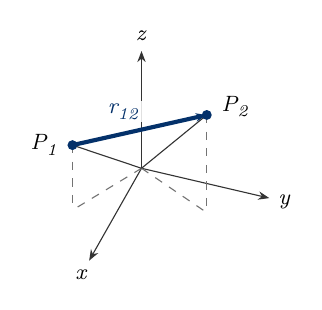
\begin{tikzpicture}[line join=round]
\draw[-{Stealth[length=4pt]},black!80] (1.381,-1.939) -- (0.716,-3.112);
\node[,inner sep=1pt,font=\footnotesize] at (0.619,-3.285) {\textit{x}};
\draw[-{Stealth[length=4pt]},black!80] (1.381,-1.939) -- (3.004,-2.318);
\node[,inner sep=1pt,font=\footnotesize] at (3.197,-2.363) {\textit{y}};
\draw[-{Stealth[length=4pt]},black!80] (1.381,-1.939) -- (1.381,-0.450);
\node[,inner sep=1pt,font=\footnotesize] at (1.381,-0.252) {\textit{z}};
\draw[black!55,dashed] (0.504,-1.645) -- (0.504,-2.471);
\draw[black!55,dashed] (1.381,-1.939) -- (0.504,-2.471);
\draw[black!80] (1.381,-1.939) -- (0.504,-1.645);
\draw[black!55,dashed] (2.210,-1.262) -- (2.210,-2.502);
\draw[black!55,dashed] (1.381,-1.939) -- (2.210,-2.502);
\draw[black!80] (1.381,-1.939) -- (2.210,-1.262);
\draw[-{Stealth[length=4pt]},FAUblue,line width=1.5pt] (0.504,-1.645) -- (2.210,-1.262);
\fill[FAUblue] (0.504,-1.645) circle (0.063);
\fill[FAUblue] (2.210,-1.262) circle (0.063);
\node[anchor=east,fill=white,fill opacity=0.85,text opacity=1,inner sep=1pt,font=\footnotesize] at (0.360,-1.645) {\textit{P\textsubscript{1}}};
\node[anchor=west,fill=white,fill opacity=0.85,text opacity=1,inner sep=1pt,font=\footnotesize] at (2.354,-1.154) {\textit{P\textsubscript{2}}};
\node[anchor=east,text=FAUblue,fill=white,fill opacity=0.85,text opacity=1,inner sep=1pt,font=\footnotesize] at (1.393,-1.219) {\textit{r\textsubscript{12}}};
\end{tikzpicture}\par\smallskip{\small\raggedright \textbf{Endpoint minus start.} The position vectors of P\textsubscript{1} = (2, \ensuremath{-}1, 2) and P\textsubscript{2} = (1, 2, 3) run from the origin; the displacement \textit{r}\textsubscript{12} (blue) runs from P\textsubscript{1} to P\textsubscript{2}, so \textit{r}\textsubscript{12} = \textit{r}\textsubscript{P2} \ensuremath{-} \textit{r}\textsubscript{P1}. The dashed lines drop each point onto the xy-plane.\par}\end{minipage}
\end{center}

\begin{keepsection}
\Needspace{7\baselineskip}
\subsection{2a: Displacement from P\textsubscript{1} to P\textsubscript{2}}

\Needspace{4\baselineskip}
Try first: subtract the starting point coordinates from the ending point coordinates, component by component.

\nopagebreak[4]{\small\itshape Answers: see “Task 2: Cartesian coordinate system” under Answers at the end.}
\end{keepsection}

\begin{keepsection}
\Needspace{6\baselineskip}
\subsection{2b: Magnitude of r = \ensuremath{-}e\textsubscript{x} + 3e\textsubscript{y} + e\textsubscript{z}}

\Needspace{3\baselineskip}
Try first: square each perpendicular component, add them, then take the positive square root.

\nopagebreak[4]{\small\itshape Answers: see “Task 2: Cartesian coordinate system” under Answers at the end.}
\end{keepsection}

\begin{keepsection}
\Needspace{7\baselineskip}
\subsection{2c: Unit vector in the direction of r}

\Needspace{4\baselineskip}
Try first: divide the vector by its magnitude; this preserves its direction and makes its length one.

\nopagebreak[4]{\small\itshape Answers: see “Task 2: Cartesian coordinate system” under Answers at the end.}
\end{keepsection}
\end{keepsection}

\begin{keepsection}
\Needspace{9\baselineskip}
\section{Task 3: Coordinate systems}

\Needspace{6\baselineskip}
Use the standard spherical convention in this course: φ is the azimuth in the xy-plane from +x, and ϑ is the polar angle down from +z.

\textbf{Connected topic:} Flux and Gauss’s law (§1.10) uses spherical coordinates for radial fields and spherical surfaces.

\begin{keepsection}
\Needspace{7\baselineskip}
\subsection{3a: Convert the position vector to spherical coordinates}

\Needspace{4\baselineskip}
Try first: find the distance from the origin, keep the given azimuth, and use the ratio of cylindrical radius to height to find the polar angle.

\nopagebreak[4]{\small\itshape Answers: see “Task 3: Coordinate systems” under Answers at the end.}
\end{keepsection}

\begin{keepsection}
\Needspace{7\baselineskip}
\subsection{3b: Complete the spherical unit-vector table}

\Needspace{4\baselineskip}
Try first: remember that φ locates the projection in the xy-plane and ϑ measures down from +z. At the z-axis, azimuth is undefined.

\nopagebreak[4]{\small\itshape Answers: see “Task 3: Coordinate systems” under Answers at the end.}
\end{keepsection}
\end{keepsection}


\clearpage
\section{Answers}
\begin{keepsection}\subsection{Task 1: Convert units}

\begin{workedbox}{1a–f \ensuremath{\cdot} Prefix conversions}
\Needspace{14\baselineskip}
\begin{enumerate}
\item \Needspace{4\baselineskip}
\textbf{1a.} The decimal 0.000011 is 11 \ensuremath{\times} 10\textsuperscript{\ensuremath{-}6}. The prefix micro (μ) means 10\textsuperscript{\ensuremath{-}6}:

\Needspace{4\baselineskip}
\begin{equation*}{C}\, =\, 0.000011\, \mathrm{F}\, =\, 11\, \times \, 10^{-6}\, \mathrm{F}\end{equation*}

\Needspace{4\baselineskip}
\begin{equation*}{C}\, =\, 11\, μ\mathrm{F}\end{equation*}

\textbf{Check:} 11 μF is 0.000011 F.
\item \Needspace{4\baselineskip}
\textbf{1b.} Multiply the mantissas first: 47.47 \ensuremath{\times} 10\textsuperscript{5} = 4.747 \ensuremath{\times} 10\textsuperscript{6}. Mega (M) means 10\textsuperscript{6}:

\Needspace{4\baselineskip}
\begin{equation*}{R}\, =\, 4.747\, \mathrm{M}Ω\end{equation*}

\textbf{Check:} 4.747 MΩ = 4,747,000 Ω = 47.47 \ensuremath{\times} 100,000 Ω.
\item \Needspace{5\baselineskip}
\textbf{1c.} Combine the decimal factor and the given power: 0.062 \ensuremath{\times} 10\textsuperscript{\ensuremath{-}3} = 62 \ensuremath{\times} 10\textsuperscript{\ensuremath{-}6}. Micro means 10\textsuperscript{\ensuremath{-}6}:

\Needspace{4\baselineskip}
\begin{equation*}{L}\, =\, 62\, μ\mathrm{H}\end{equation*}

\textbf{Check:} 62 μH = 0.000062 H.
\item \Needspace{4\baselineskip}
\textbf{1d.} Kilo (k) means 10\textsuperscript{3}, and 30,000 = 30 \ensuremath{\times} 10\textsuperscript{3}:

\Needspace{4\baselineskip}
\begin{equation*}{U}\, =\, 30\, \text{kV}\end{equation*}

\textbf{Check:} 30 kV = 30,000 V.
\item \Needspace{4\baselineskip}
\textbf{1e.} 0.88 \ensuremath{\times} 10\textsuperscript{\ensuremath{-}4} = 8.8 \ensuremath{\times} 10\textsuperscript{\ensuremath{-}5} = 88 \ensuremath{\times} 10\textsuperscript{\ensuremath{-}6}. Micro means 10\textsuperscript{\ensuremath{-}6}:

\Needspace{4\baselineskip}
\begin{equation*}{I}\, =\, 88\, μ\mathrm{A}\end{equation*}

\textbf{Check:} 88 μA = 0.000088 A.
\item \Needspace{4\baselineskip}
\textbf{1f.} 1265 \ensuremath{\times} 10\textsuperscript{6} = 1.265 \ensuremath{\times} 10\textsuperscript{9}. Giga (G) means 10\textsuperscript{9}:

\Needspace{4\baselineskip}
\begin{equation*}{P}\, =\, 1.265\, \text{GW}\end{equation*}

\textbf{Check:} 1.265 GW = 1,265,000,000 W.
\end{enumerate}
\end{workedbox}

\end{keepsection}
\begin{keepsection}\subsection{Task 2: Cartesian coordinate system}

\begin{workedbox}{2a \ensuremath{\cdot} Displacement vector}
\Needspace{9\baselineskip}
\begin{enumerate}
\item \Needspace{4\baselineskip}
A vector from point 1 to point 2 is the endpoint position minus the starting position:

\begin{equation*}{r}_{12}\, =\, {r}_{\mathrm{P}2}\, -\, {r}_{\mathrm{P}1}\end{equation*}
\item \Needspace{4\baselineskip}
Subtract each matching coordinate:

\Needspace{4\baselineskip}
\begin{equation*}{r}_{12}\, =\, (1\, -\, 2,\, 2\, -\, (-1),\, 3\, -\, 2)\end{equation*}

\Needspace{4\baselineskip}
\begin{equation*}{r}_{12}\, =\, (-1,\, 3,\, 1)\end{equation*}

\begin{equation*}{r}_{12}\, =\, -{e}_{\mathrm{x}}\, +\, 3{e}_{\mathrm{y}}\, +\, {e}_{\mathrm{z}}\end{equation*}
\item \Needspace{6\baselineskip}
\textbf{Result:} the displacement is (\ensuremath{-}1, 3, 1) coordinate units. The negative x-component means the motion is toward decreasing x; the y and z components are positive.

\textbf{Check:} adding the displacement to P\textsubscript{1} gives (2, \ensuremath{-}1, 2) + (\ensuremath{-}1, 3, 1) = (1, 2, 3), the stated endpoint.
\end{enumerate}
\end{workedbox}

\end{keepsection}
\begin{keepsection}\subsection{Task 2: Cartesian coordinate system}

\begin{workedbox}{2b \ensuremath{\cdot} Vector magnitude}
\Needspace{6\baselineskip}
\begin{enumerate}
\item \Needspace{4\baselineskip}
For Cartesian components, the length follows from the three-dimensional Pythagorean theorem:

\begin{equation*}|{r}|\, =\, \sqrt{{r}_{{x}}^{2}\, +\, {r}_{{y}}^{2}\, +\, {r}_{{z}}^{2}}\end{equation*}
\item \Needspace{4\baselineskip}
Here the components are (\ensuremath{-}1, 3, 1), so:

\Needspace{4\baselineskip}
\begin{equation*}|{r}|\, =\, \sqrt{(-1)^{2}\, +\, 3^{2}\, +\, 1^{2}}\end{equation*}

\Needspace{4\baselineskip}
\begin{equation*}|{r}|\, =\, \sqrt{11}\, \approx \, 3.32\end{equation*}

\Needspace{4\baselineskip}
\textbf{Result:} |\textit{r}| = \ensuremath{\sqrt{11}} coordinate units.

\textbf{Check:} a magnitude cannot be negative, and its square is 1 + 9 + 1 = 11.
\end{enumerate}
\end{workedbox}

\end{keepsection}
\begin{keepsection}\subsection{Task 2: Cartesian coordinate system}

\begin{workedbox}{2c \ensuremath{\cdot} Normalised direction}
\Needspace{5\baselineskip}
\begin{enumerate}
\item \Needspace{4\baselineskip}
The unit vector is the original vector divided by its positive length:

\begin{equation*}{e}_{\mathrm{r}}\, =\, \dfrac{{r}}{|{r}|}\end{equation*}
\item \Needspace{4\baselineskip}
Divide the vector from 2a by its magnitude from 2b:

\Needspace{4\baselineskip}
\begin{equation*}{e}_{\mathrm{r}}\, =\, \dfrac{-{e}_{\mathrm{x}}\, +\, 3{e}_{\mathrm{y}}\, +\, {e}_{\mathrm{z}}}{\sqrt{11}}\end{equation*}

\Needspace{4\baselineskip}
\textbf{Result:} \textit{e}\textsubscript{r} = {\small\ensuremath{\dfrac{-1,\, 3,\, 1}{\sqrt{11}}}}.

\textbf{Check:} its length is \ensuremath{\sqrt{\dfrac{1\, +\, 9\, +\, 1}{11}}} = 1.
\end{enumerate}
\end{workedbox}

\end{keepsection}
\begin{keepsection}\subsection{Task 3: Coordinate systems}

\begin{workedbox}{3a \ensuremath{\cdot} Cylindrical to spherical}
\Needspace{14\baselineskip}
\begin{enumerate}
\item \Needspace{5\baselineskip}
The cylindrical components are \textit{ρ} = 5, \textit{z} = 2, and φ = 45°. The spherical radius is the distance from the origin:

\begin{equation*}{r}\, =\, \sqrt{{ρ}^{2}\, +\, {z}^{2}}\, =\, \sqrt{25\, +\, 4}\, =\, \sqrt{29}\end{equation*}
\item \Needspace{5\baselineskip}
\textit{ϑ} is measured from +z, so its tangent is opposite over adjacent = {\small\ensuremath{\dfrac{ρ}{\mathrm{z}}}}. The point is above the xy-plane, hence \textit{ϑ} is in the first quadrant:

\begin{equation*}{ϑ}\, =\, \arctan \left(\dfrac{{ρ}}{{z}}\right)\, =\, \arctan \left(\dfrac{5}{2}\right)\, \approx \, 68.2°\end{equation*}
\item \Needspace{5\baselineskip}
The azimuth remains the supplied angle, φ = 45°. State the spherical coordinates by name so the angle order is clear:

\Needspace{4\baselineskip}
\begin{equation*}{r}\, =\, \sqrt{29}\end{equation*}

\Needspace{4\baselineskip}
\begin{equation*}{φ}\, =\, 45°\end{equation*}

\begin{equation*}{ϑ}\, \approx \, 68.2°\end{equation*}
\item \Needspace{5\baselineskip}
As a position vector, \textit{r} = \textit{r}\textit{e}\textsubscript{r}. Since \textit{ϑ} = arctan({\small\ensuremath{\dfrac{5}{2}}}), sin\textit{ϑ} = {\small\ensuremath{\dfrac{5}{\sqrt{29}}}} and cos\textit{ϑ} = {\small\ensuremath{\dfrac{2}{\sqrt{29}}}}, so the vector has no \textit{e}\textsubscript{ϑ} component:

\Needspace{4\baselineskip}
\begin{equation*}{r}\, =\, \sqrt{29}\, {e}_{\mathrm{r}}\end{equation*}

\Needspace{8\baselineskip}
\textbf{Check:} its cylindrical projection is \textit{r} sinϑ = 5 and its z-component is \textit{r} cosϑ = 2.

\Needspace{14\baselineskip}
\begin{center}
\begin{minipage}[t]{0.950\linewidth}\centering
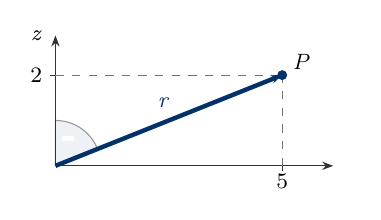
\begin{tikzpicture}[line join=round]
\filldraw[draw=black!40,fill=Paperblue] (1.471,-2.090) -- (1.465,-2.077) -- (1.460,-2.064) -- (1.453,-2.051) -- (1.447,-2.038) -- (1.440,-2.026) -- (1.433,-2.013) -- (1.426,-2.001) -- (1.418,-1.989) -- (1.410,-1.977) -- (1.402,-1.965) -- (1.393,-1.954) -- (1.385,-1.943) -- (1.375,-1.932) -- (1.366,-1.921) -- (1.356,-1.910) -- (1.347,-1.900) -- (1.336,-1.890) -- (1.326,-1.880) -- (1.315,-1.871) -- (1.305,-1.861) -- (1.293,-1.852) -- (1.282,-1.844) -- (1.271,-1.835) -- (1.259,-1.827) -- (1.247,-1.819) -- (1.235,-1.812) -- (1.223,-1.804) -- (1.210,-1.797) -- (1.197,-1.791) -- (1.185,-1.784) -- (1.172,-1.778) -- (1.159,-1.773) -- (1.145,-1.767) -- (1.132,-1.762) -- (1.118,-1.758) -- (1.105,-1.753) -- (1.091,-1.749) -- (1.077,-1.746) -- (1.063,-1.742) -- (1.050,-1.739) -- (1.035,-1.737) -- (1.021,-1.734) -- (1.007,-1.732) -- (0.993,-1.731) -- (0.979,-1.730) -- (0.965,-1.729) -- (0.950,-1.728) -- (0.936,-1.728) -- (0.936,-2.304) -- (0.936,-2.304) -- (0.936,-2.304) -- (0.936,-2.304) -- (0.936,-2.304) -- (0.936,-2.304) -- (0.936,-2.304) -- (0.936,-2.304) -- (0.936,-2.304) -- (0.936,-2.304) -- (0.936,-2.304) -- (0.936,-2.304) -- (0.936,-2.304) -- (0.936,-2.304) -- (0.936,-2.304) -- (0.936,-2.304) -- (0.936,-2.304) -- (0.936,-2.304) -- (0.936,-2.304) -- (0.936,-2.304) -- (0.936,-2.304) -- (0.936,-2.304) -- (0.936,-2.304) -- (0.936,-2.304) -- (0.936,-2.304) -- (0.936,-2.304) -- (0.936,-2.304) -- (0.936,-2.304) -- (0.936,-2.304) -- (0.936,-2.304) -- (0.936,-2.304) -- (0.936,-2.304) -- (0.936,-2.304) -- (0.936,-2.304) -- (0.936,-2.304) -- (0.936,-2.304) -- (0.936,-2.304) -- (0.936,-2.304) -- (0.936,-2.304) -- (0.936,-2.304) -- (0.936,-2.304) -- (0.936,-2.304) -- (0.936,-2.304) -- (0.936,-2.304) -- (0.936,-2.304) -- (0.936,-2.304) -- (0.936,-2.304) -- (0.936,-2.304) -- (0.936,-2.304) -- cycle;
\draw[-{Stealth[length=4pt]},black!80] (0.936,-2.304) -- (4.464,-2.304);
\node[anchor=west,fill=white,fill opacity=0.85,text opacity=1,inner sep=1pt,font=\footnotesize] at (4.554,-2.484) {\textit{ρ}};
\draw[-{Stealth[length=4pt]},black!80] (0.936,-2.304) -- (0.936,-0.648);
\node[anchor=east,fill=white,fill opacity=0.85,text opacity=1,inner sep=1pt,font=\footnotesize] at (0.810,-0.648) {\textit{z}};
\draw[black!80] (3.816,-2.232) -- (3.816,-2.376);
\node[fill=white,fill opacity=0.85,text opacity=1,inner sep=1pt,font=\footnotesize] at (3.816,-2.502) {5};
\draw[black!80] (0.864,-1.152) -- (1.008,-1.152);
\node[anchor=east,fill=white,fill opacity=0.85,text opacity=1,inner sep=1pt,font=\footnotesize] at (0.810,-1.152) {2};
\draw[black!55,dashed] (3.816,-2.304) -- (3.816,-1.152);
\draw[black!55,dashed] (0.936,-1.152) -- (3.816,-1.152);
\draw[-{Stealth[length=4pt]},FAUblue,line width=1.6pt] (0.936,-2.304) -- (3.816,-1.152);
\fill[FAUblue] (3.816,-1.152) circle (0.063);
\node[fill=white,fill opacity=0.85,text opacity=1,inner sep=1pt,font=\footnotesize] at (1.094,-1.958) {\textit{ϑ}};
\node[anchor=east,text=FAUblue,fill=white,fill opacity=0.85,text opacity=1,inner sep=1pt,font=\footnotesize] at (2.430,-1.508) {\textit{r}};
\node[anchor=west,fill=white,fill opacity=0.85,text opacity=1,inner sep=1pt,font=\footnotesize] at (3.906,-0.990) {\textit{P}};
\end{tikzpicture}\par\smallskip{\small\raggedright \textbf{Cylindrical to spherical in one plane.} The vertical plane through P at φ = 45° holds ρ = 5 across and \textit{z} = 2 up. The distance \textit{r} = \ensuremath{\sqrt{29}} is the hypotenuse, and ϑ is the angle down from the \textit{z}-axis, so tan ϑ = {\small\ensuremath{\dfrac{ρ}{{z}}}}.\par}\end{minipage}
\end{center}
\end{enumerate}
\end{workedbox}

\end{keepsection}
\begin{keepsection}\subsection{Task 3: Coordinate systems}

\begin{workedbox}{3b \ensuremath{\cdot} Unit vectors and spherical angles}
\Needspace{14\baselineskip}
\begin{enumerate}
\item \Needspace{4\baselineskip}
For a unit direction, take its projection onto each Cartesian basis vector:

\Needspace{4\baselineskip}
\begin{equation*}{e}_{\mathrm{r}}\, \cdot \, {e}_{\mathrm{x}}\, =\, \sin {ϑ}\, \cos {φ}\end{equation*}

\Needspace{4\baselineskip}
\begin{equation*}{e}_{\mathrm{r}}\, \cdot \, {e}_{\mathrm{y}}\, =\, \sin {ϑ}\, \sin {φ}\end{equation*}

\Needspace{5\baselineskip}
\begin{equation*}{e}_{\mathrm{r}}\, \cdot \, {e}_{\mathrm{z}}\, =\, \cos {ϑ}\end{equation*}

Evaluate these three components for each listed direction. At either pole (\ensuremath{\pm}\textit{e}\textsubscript{z}), φ can be chosen arbitrarily because the projection into the xy-plane has zero length.
\item \Needspace{17\baselineskip}
The completed entries are:

\Needspace{10\baselineskip}
\begin{center}\small\begin{tabularx}{\linewidth}{>{\raggedright\arraybackslash}X>{\raggedright\arraybackslash}X>{\raggedright\arraybackslash}X}\toprule
\textbf{Cartesian unit vector} & \textbf{\textit{φ}} & \textbf{\textit{ϑ}} \\ \midrule
\textit{e}\textsubscript{z} & any (the sheet’s *) & 0° \\
\ensuremath{-}\textit{e}\textsubscript{z} & any (the sheet’s *) & 180° \\
\textit{e}\textsubscript{x} & 0° & 90° \\
\ensuremath{-}\textit{e}\textsubscript{x} & 180° & 90° \\
\textit{e}\textsubscript{y} & 90° & 90° \\
\ensuremath{-}\textit{e}\textsubscript{y} & 270° & 90° \\
{\small\ensuremath{\dfrac{{e}_{\mathrm{x}}\, +\, {e}_{\mathrm{y}}}{\sqrt{2}}}} & 45° & 90° \\
{\small\ensuremath{\dfrac{{e}_{\mathrm{x}}\, -\, {e}_{\mathrm{z}}}{\sqrt{2}}}} & 0° & 135° \\
{\small\ensuremath{\dfrac{{e}_{\mathrm{y}}\, +\, {e}_{\mathrm{z}}}{\sqrt{2}}}} & 90° & 45° \\
\bottomrule\end{tabularx}\end{center}
\item \Needspace{6\baselineskip}
For the last three rows, substitute the angles into the unit-vector formula. For example, φ = 0° and ϑ = 135° gives (sin135°, 0, cos135°) = ({\small\ensuremath{\dfrac{1}{\sqrt{2}}}}, 0, \ensuremath{-}{\small\ensuremath{\dfrac{1}{\sqrt{2}}}}).

\textbf{Check:} every listed Cartesian vector has unit length. Angles differing by 360° represent the same azimuth, so \ensuremath{-}90° is equivalent to 270°.
\end{enumerate}
\end{workedbox}

\end{keepsection}

\vfill{\small Personal worked-solution guide based on the supplied EE1 Tutorial Task sheet, written in my own words; no tutorial text or figures are reproduced. Not an official FAU publication; check course details against current material. Made by \textbf{Thanate Amornjiraporn (Focus)}.}

\end{document}
